\section{Auswertung}
\label{sec:Auswertung}

\subsection{Entladung eines Kondensators}

Die aufgenommenen Wertepaare finden sich in Tabelle \ref{tab:Messdaten1}.

\begin{table}
\centering
\caption{Messdaten zur Entladekurve}
\label{tab:Messdaten1}
\sisetup{table-format=2.1}
\begin{tabular}{c c}
\toprule
$t \,/\, \si{\milli\second}$ & $U_C \,/\, \si{\volt}$\\
\midrule
0,00 & 100\\
0,26 &  82\\
0,50 &  70\\
0,76 &  58\\
1,00 &  46\\
1,26 &  38\\
1,50 &  30\\
2,00 &  20\\
3,00 &   6\\
4,10 &   0\\
\bottomrule
\end{tabular}
\end{table} 

Die Wertepaare werden in einem halblogarithmischen Diagramm dargestellt. Dazu 
wird eine lineare Regression mittels Python und matplotlib durchgeführt. Das 
entstandene Diagramm ist in Abbildung \ref{fig:plot1} zu finden. 

\begin{figure}
  \centering
  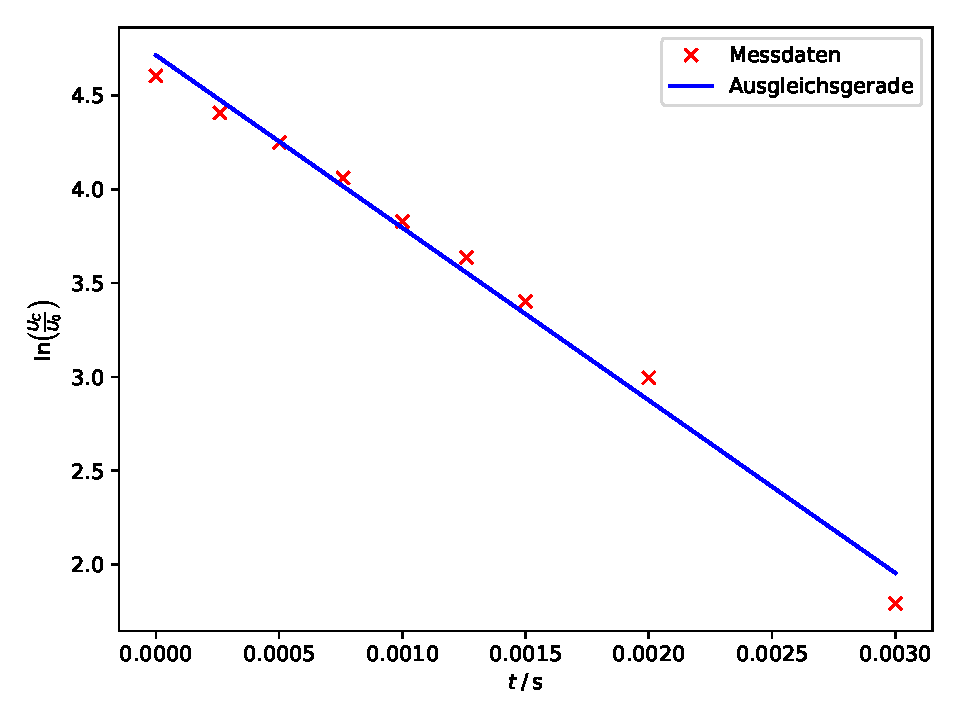
\includegraphics[scale=0.8]{content/plot1.pdf}
  \caption{Lineare Regression zur Bestimmung der Zeitkonstanten mithilfe
  der Entladekurve}
  \label{fig:plot1}
\end{figure}

Die lineare Ausgleichsrechnung der logarithmierten Daten mit $\ln{\left(U_C\right)}=ax+b$ 
ergibt folgende Regressionsparameter: 

\begin{align*}
a &= \SI{-919.67+-45.48}{\per\second},\\
b &= \num{4.71+-0.07}.
\end{align*}

Durch Vergleich mit der Formel \eqref{eqn:ent} ergibt sich für die Zeitkonstante:

\begin{equation*}
RC = -\frac{1}{a} = \SI{1.09+-0.05}{\milli\second}.
\end{equation*}

\subsection{Frequenzabhängigkeit der Amplitude}

In diesem Versuchsteil wird die Frequenzabhängigkeit der Amplitude der 
Kondensatorspannung $U_C$ untersucht. Hierzu wird diese für verschiedene 
Frequenzen $f$ gemessen. Die Messwerte finden sich in Tabelle \ref{tab:Messdaten2}.
Außerdem wird die Amplitude der Generatorspannung zu $U_0=\SI{51.6}{\volt}$ gemessen und 
so das Verhältnis $\frac{A}{U_0}$ für jeden Messwert bestimmt. 

\begin{table}
\centering
\caption{Messdaten zur Frequenzabhängigkeit der Amplitude}
\label{tab:Messdaten2}
\sisetup{table-format=2.1}
\begin{tabular}{c c c}
\toprule
$f \,/\, \si{\hertz}$ & $A \,/\, \si{\volt}$ & $\frac{A}{U_0}$ \\
\midrule
   10 & 49,60 & 0.961\\
   20 & 49,20 & 0.953\\
   30 & 48,00 & 0.930\\
   40 & 46,40 & 0.899\\
   50 & 45,20 & 0.876\\
   60 & 43,60 & 0.845\\
   70 & 42,00 & 0.814\\
   80 & 40,70 & 0.789\\
   90 & 39,20 & 0.760\\
  100 & 37,20 & 0.721\\
  200 & 29,40 & 0.570\\
  300 & 17,60 & 0.341\\
  400 & 13,40 & 0.260\\
  500 & 11,00 & 0.213\\
  600 &  9,10 & 0.176\\
  700 &  7,80 & 0.151\\
  800 &  6,90 & 0.134\\
  900 &  6,30 & 0.122\\
 1000 &  5,60 & 0.109\\
 2000 &  2,76 & 0.053\\
 3000 &  1,84 & 0.036\\
 4000 &  1,40 & 0.027\\
 5000 &  1,12 & 0.022\\
 6000 &  0,92 & 0.018\\
 7000 &  0,80 & 0.016\\
 8000 &  0,71 & 0.014\\
 9000 &  0,62 & 0.012\\
10000 &  0,56 & 0.011\\
\bottomrule
\end{tabular}
\end{table} 

In Abbildung \ref{fig:plot2} werden die gemessenen mit der Erregerspannung normierten
Amplituden gegen die Frequenz der Erregerspannung halblogarithmisch
aufgetragen. 

\begin{figure}
  \centering
  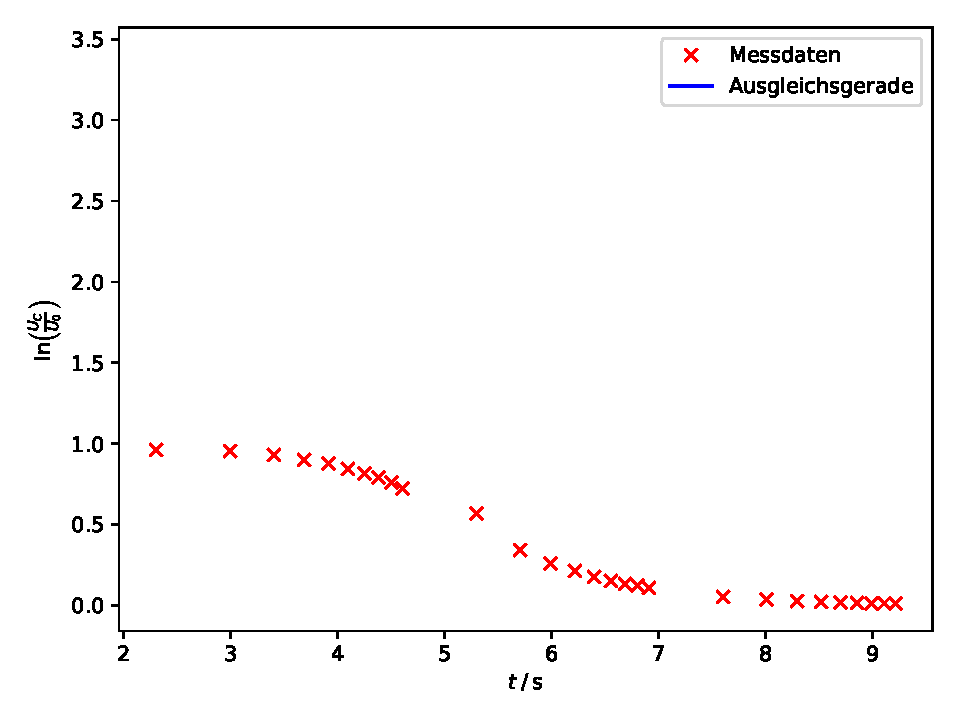
\includegraphics[scale=0.8]{content/plot2.pdf}
  \caption{Normierte Kondensatoramplituden}
  \label{fig:plot2}
\end{figure}

Mittels eines Fits der Form

\begin{equation*}
f = \frac{1}{\sqrt{1+x²m²}}+b,
\end{equation*}

werden die Messwerte gefittet. Die Parameter ergeben sich dabei zu

\begin{align*}
m &= \num{-8.64+-0.34e-3},\\
b &= \num{-14.90+-6.91e-3}.
\end{align*}

Somit ergibt sich nach Formel \eqref{eqn:Amplitude} die Zeitkonstante $RC$ zu

\begin{equation*}
RC = \SI{8.64+-0.34}{\milli\second}. 
\end{equation*}

\subsection{Frequenzabhängigkeit der Phasenverschiebung}

In diesem Versuchsteil wird die Frequenzabhängigkeit der Phasenverschiebung
zwischen der Kondensator- und Generatorspannung untersucht. Über die Frequenz 
wird dabei die jeweilige Periodendauer nach $T= \frac{1}{f}$ bestimmt. Außerdem
wird aus dem abgelesenem zeitlichen Abstand $\Delta t$ zwischen den beiden 
Maxima und der Periodendauer die Phasenverschiebung gemäß 

\begin{equation*}
\phi = \frac{\Delta t}{T} 2 \pi
\end{equation*}

bestimmt. 
Die Messdaten und die daraus bestimmten Größen sind in Tabelle \ref{tab:Messdaten3} zu finden. 

\begin{table}
\centering
\caption{Messdaten zur Frequenzabhängigkeit der Phasenverschiebung}
\label{tab:Messdaten3}
\sisetup{table-format=2.1}
\begin{tabular}{c c c c}
\toprule
$f \,/\, \si{\hertz}$ & $T=\frac{1}{f} \,/\, \si{\milli\second}$ 
&$\Delta t \,/\, \si{\milli\second}$ & $\phi \,/\, \si{\radian}$\\
\midrule
   10 & 100,00 & 12,000 & 0,75\\
   20 &  50,00 &  4,200 & 0,53\\
   30 &  33,33 &  2,600 & 0,49\\
   40 &  25,00 &  1,900 & 0,48\\
   50 &  20,00 &  1,800 & 0,57\\
   60 &  16,67 &  1,700 & 0,64\\
   70 &  14,29 &  1,640 & 0,72\\
   80 &  12,50 &  1,440 & 0,72\\
   90 &  11,11 &  1,400 & 0,79\\
  100 &  10,00 &  1,280 & 0,80\\
  200 &   5,00 &  0,780 & 0,98\\
  300 &   3,33 &  0,640 & 1,21\\
  400 &   2,50 &  0,560 & 1,41\\
  500 &   2,00 &  0,440 & 1,38\\
  600 &   1,67 &  0,390 & 1,47\\
  700 &   1,43 &  0,340 & 1,50\\
  800 &   1,25 &  0,280 & 1,41\\
  900 &   1,11 &  0,270 & 1,53\\
 1000 &   1,00 &  0,240 & 1,51\\
 2000 &   0,50 &  0,116 & 1,46\\
 3000 &   0,33 &  0,080 & 1,51\\
 4000 &   0,25 &  0,060 & 1,51\\
 5000 &   0,20 &  0,048 & 1,51\\
 6000 &   0,17 &  0,041 & 1,55\\
 7000 &   0,14 &  0,035 & 1,54\\
 8000 &   0,13 &  0,031 & 1,56\\
 9000 &   0,11 &  0,027 & 1,53\\
10000 &   0,10 &  0,024 & 1,51\\
\bottomrule
\end{tabular}
\end{table} 

Diese Daten werden ebenfalls halblogarithmisch gegen die Erregerfrequenz 
aufgetragen. Das Resultat ist in Abbildung \ref{fig:plot3} zu sehen. 

\begin{figure}
  \centering
  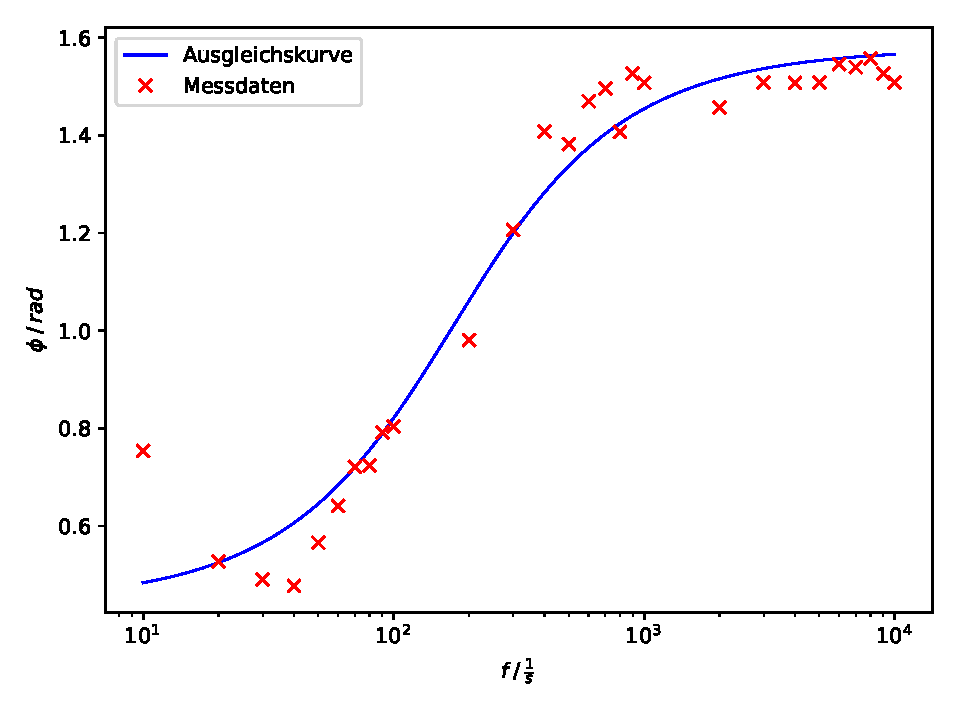
\includegraphics[scale=0.8]{content/plot3.pdf}
  \caption{Phasenverschiebungen}
  \label{fig:plot3}
\end{figure}

Es wird eine Funktion der Art 

\begin{equation*}
f = a\cdot\text{arctan}(mx)+b,
\end{equation*}

identisch \eqref{eqn:Phase}, gefittet. Die Parameter ergeben sich zu 

\begin{align*}
a &= \num{-0.72+-0.03},\\
m &= \num{-0.0058+-0.0009},\\
b &= \num{0.44+-0.05}.
\end{align*}

Die nicht-lineare Ausgleichsrechnung lässt somit auf den Wert

\begin{equation*}
RC = \SI{5.8+-0.9}{\milli\second}
\end{equation*}

schließen.
Mit letzterem kann ein Polarplot erstellt werden. Der Winkel $\phi$ beschreibt 
die Phasenverschiebung, der Radius hingegegen die normierte Amplitude der
Kondensatorspannung. Es resultiert der Polarplot in Abbildung mit 
$RC = \SI{5.8+-0.9}{\milli\second}$.

\begin{figure}
  \centering
  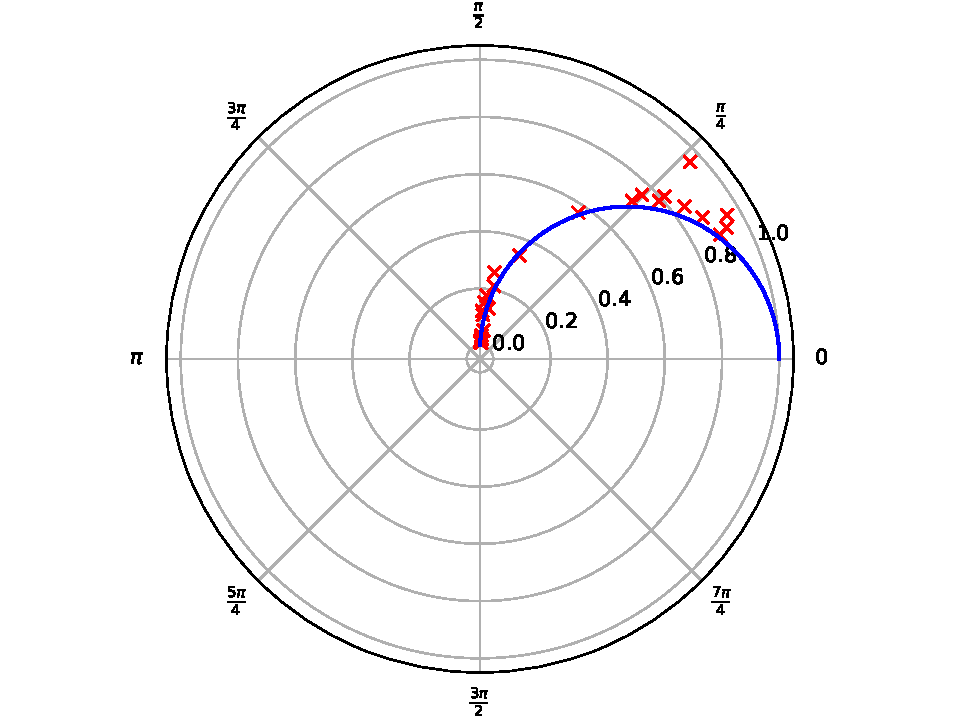
\includegraphics[scale=0.8]{content/plot4.pdf}
  \caption{Polarplot}
  \label{fig:plot4}
\end{figure}

Es wurden mehrere Probewerte eingezeichnet.

\subsection{Der RC-Kreis als Integrator}

In diesem Versuchsteil wird gezeigt, dass der RC-Kreis als Integrator arbeiten 
kann, wenn $\omega \gg \frac{1}{RC}$. Dazu wird dieser mit einer Rechtecks-, 
Sinus- und Dreiecksspannung gespeist und sowohl die Ursprungssignale als auch 
die integrierten Signale auf dem Oszilloskop angezeigt. Um die geforderte 
Bedingung an $\omega$ zu gewährleisten, werden Frequenzen von etwa \SI{5}{\kilo\hertz}
verwendet. 
Die Ursprungssignale und die integrierten Signale sind jeweils in den Abbildungen 
\ref{fig:Sinus}, \ref{fig:Dreieck} und \ref{fig:Rechteck} zu erkennen. Dabei ist
die mit dem Cursor erfasste Funktion stets das integrierte Signal

\begin{figure}
  \centering
  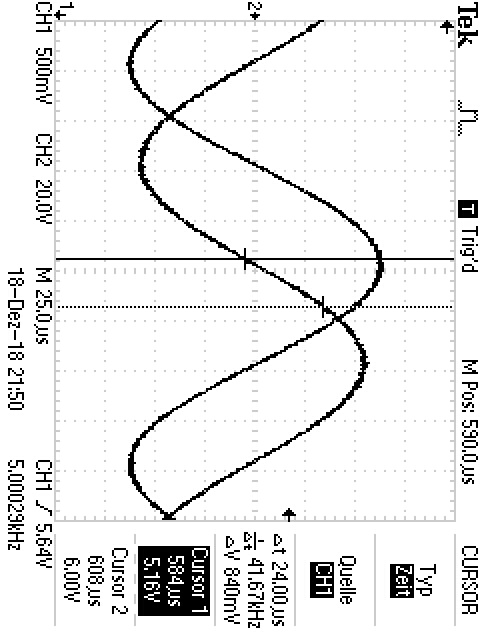
\includegraphics[angle=90, scale=0.8]{content/Sinus.jpg} 
  \caption{Integration eines Sinussignals durch das RC-Glied}
  \label{fig:Sinus}
\end{figure}

\begin{figure}
  \centering
  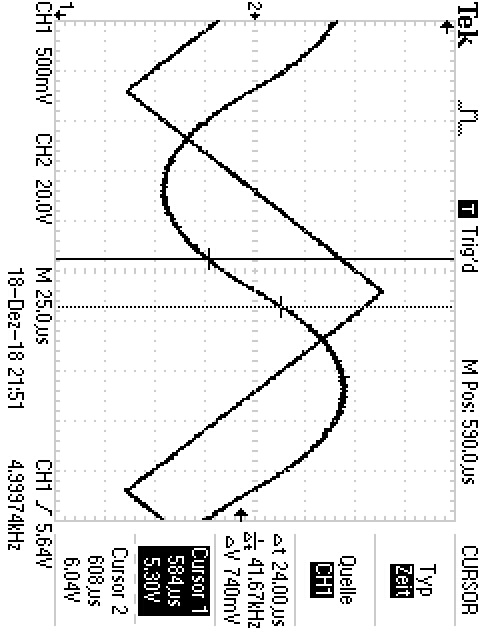
\includegraphics[angle=90, scale=0.8]{content/Dreieck.jpg}
  \caption{Integration eines Dreiecksignals durch das RC-Glied}
  \label{fig:Dreieck}
\end{figure}

\begin{figure}
  \centering
  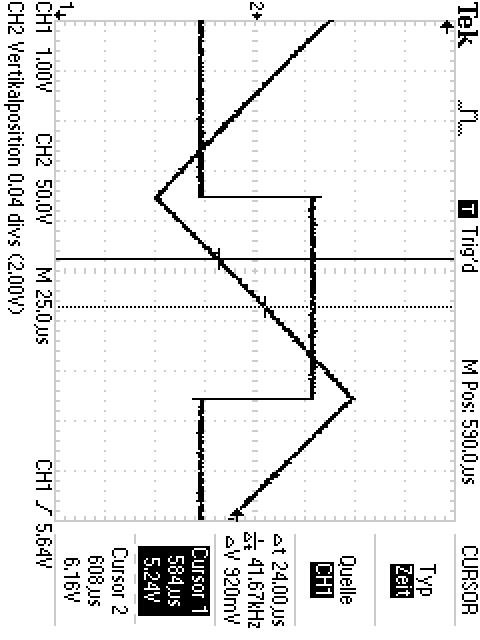
\includegraphics[angle=90, scale=0.8]{content/Rechteck.jpg}
  \caption{Integration eines Rechtecksignals durch das RC-Glied}
  \label{fig:Rechteck}
\end{figure}
